%%This file was created by Wu Shin Ting for the first edition of EADCA (Nov/2007)
%%Revised by Wu Sin Ting in Mai/2022
\documentclass[11pt]{article}
\usepackage{eadca-template}
\usepackage[plain]{algorithm}

\usepackage[brazil,english]{babel}
\usepackage[utf8]{inputenc}
\usepackage[T1]{fontenc}

\usepackage{graphicx,url}
\usepackage[hang]{subfigure}
\DeclareGraphicsExtensions{.png,PNG,.pdf,.PDF}


\title{Instruções para Autores}

\author{Autores \and Orientador(es)}

\email{\{autores, orientador@dca.fee.unicamp.br\}}

\address{Departamento de Engenharia de Computação e Automação (DCA) \\
Faculdade de Engenharia Elétrica e de Computação (FEEC) \\
Universidade Estadual de Campinas (Unicamp) \\
Campinas, SP, Brasil \\
}
\begin{document}

\hyphenation{}
\pagestyle{fancy}

%%%%%%%%%%%%%%%%%%%%%%%%%%%%%%%%%%%%%%%%%%%%%%%%%%%%%%%%%%%%%%%%%%%%%%%%%%%%%
\selectlanguage{brazil}
\twocolumn[
\maketitle
  \thispagestyle{fancy}

  \begin{abstract}
Este artigo fornece algumas diretrizes para preparar um artigo de duas colunas. O resumo é limitado a 150 palavras. Ele deve ser uma descrição autocontida do seu trabalho, incluindo a motivação, o problema, a maneira como você planeja resolver/resolveu seu problema, resultados esperados/alcançados/na estrada e as implicações de seus resultados. É uma forma de convencer as pessoas de que vale a pena ler o restante do artigo. Citamos excepcionalmente ~\cite{Koop97} neste resumo para leitura adicional acerca elaboração de um bom resumo.    
   \end{abstract}

  \keywords{Coloque aqui palavras-chave que as pessoas que procuram seu artigo podem usar ou que podem ajudar os comitês de revisão ou editores a atribuí-lo aos revisores apropriados.}
]
%%%%%%%%%%%%%%%%%%%%%%%%%%%%%%%%%%%%%%%%%%%%%%%%%%%%%%%%%%%%%%%%%%%%%%%%%%%%%
\selectlanguage{brazil}

  \section{Introdução}
  \label{sec:introducao}

   Os trabalhos, que podem ser escritos tanto em português quanto em
   inglês, devem conter uma introdução, a sua proposta de
   pesquisa, os resultados esperados e/ou já obtidos, conclusões, uma seção
   de agradecimentos e uma lista de referências bibliográficas. Cada trabalho
   deve ter, no máximo, quatro páginas, incluindo figuras, tabelas e demais 
   itens complementares. Os tipos e tamanhos das fontes, assim como as
   margens e os diversos estilos necessários, devem corresponder aos
   apresentados neste documento.

   Na introdução, você deve expor com clareza as motivações
   subjacentes ao problema tratado em seu artigo, mostrando aos seus
   leitores a importância do tema. Se o seu trabalho se insere em um
   assunto mais amplo, pode ser interessante que você sintetize este
   assunto antes de especificar o seu problema. Um pequeno resumo
   sobre como o seu problema tem sido estudado pelos outros
   pesquisadores também pode contribuir para situar o seu
   trabalho~\cite{Blinn87}. Em alguns casos, é válido incluir na
   introdução as conjecturas ou hipóteses que ajudarão a guiar as
   suas investigações.
  %%%%%%%%%%%%%%%%%%%%%%%%%%%%%%%%%%%%%%%%%%%%%%%%%%%%%%%%%%%%%%%%%%%%%%%%%%%%%
  \section{Proposta}
  \label{sec:detalhes}

  A proposta deve ser objetiva, ou seja, nela devem ser destacadas as
  ideias-chave.  Recursos complementares, como diagramas e figuras,
  podem ajudar na explanação das suas ideias.  Fluxogramas são boas
  alternativas para apresentar um procedimento, grafos ajudam a
  visualizar as relações entre os objetos de interesse e imagens
  bonitas sempre chamam atenção.

   Ao escrever a sua proposta, procure utilizar uma linguagem clara e
   objetiva. Frases curtas e em ordem direta são mais recomendadas
   para textos científicos. Repetições de palavras ou de ideias devem
   ser evitadas. Vale lembrar que, hoje em dia, a maioria dos
   processadores de texto contém corretores ortográficos. Portanto,
   erros de grafia e digitação podem ser facilmente
   eliminados. Recomendamos a leitura do artigo do Prof. Rogério
   Lacaz-Ruiz~\cite{LR}, que dá algumas noções acerca redação de um texto
   científico.

  Nesta seção, apresentamos detalhes da formatação dos artigos do
  Encontro de Alunos e Docentes do DCA (EADCA).


\subsection{Páginas}
\label{sec:paginas}

As páginas {\bf não devem ser numeradas}. As medidas de formatação
são: folha A4; margem superior: 2,5 cm; margem inferior: 2,0 cm;
margem esquerda: 1,5 cm; margem direita: 1,5 cm. O texto deve ser em
duas colunas balanceadas no final do documento, separadas por um
espaço de 0,5 cm. O espaçamento entre o texto e o cabeçalho deve ser
0.5cm. A fonte é {\it Time News Roman\/} 11pt. Os títulos tem fonte maior, 
12pt para subseções e 13pt para seções.  A identação e o espaçamento 
entre os parágrafos são 0,8 cm e 0.2 cm, respectivamente.

A primeira página deve conter o título do trabalho, nome do autor e do
orientador, endereço dos autores, um {\it abstract\/} e um conjunto de
{\it keywords\/} em inglês. O título de cada seção ou subseção deve
estar em negrito. Procure evitar seções com uma única subseção: usualmente,
ela pode ser substituída por parágrafos sem comprometer a qualidade do texto.


\subsection{Figuras e Legendas}
\label{sec:figuras}

As figuras são, de certa forma, complementares a seu texto.  Portanto,
elas devem ser citadas, e o texto contido nelas deve ser na mesma
língua. Elas poderão ocupar uma ou duas colunas.  Abaixo de cada
figura devem ser colocados o seu número e uma legenda.  Adote uma
numeração única para o documento todo e centralize as legendas, em
consonância com o modelo da Figura~\ref{fig:forma_de_onda}, que traz o
gráfico de uma função senoidal.

  \begin{figure}[H]
        {\centering
        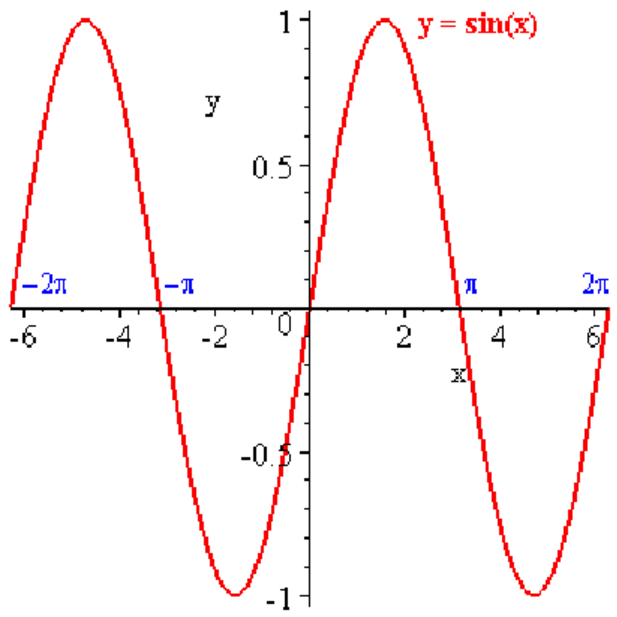
\includegraphics[height=35mm]{sin.pdf}
        \caption{Forma de onda senoidal.}
        \label{fig:forma_de_onda}\par}
  \end{figure}

\subsection{Tabelas}
\label{ssec:tabelas}

A formatação das tabelas segue a mesma recomendação das figuras.
A Tabela~\ref{tab:ex} ilustra o uso de uma tabela. Esta tabela sintetiza
o tempo, em meses, que cada grupo $G_i$ necessitou para realizar a
tarefa $T_j$.

\begin{table}[H]
  {\centering
  \begin{tabular}{|c|c|c|c|c|}
  \hline
   & $G_1$ & $G_2$ & $G_2$ & $G_3$ \\
  \hline
  $T_1$ & 2 & 4 & 6 & 8 \\
  \hline
  $T_2$ & 3 & 6 & 9 & 12 \\
  \hline
  \end{tabular}
\caption{Exemplo de uma tabela.}
\label{tab:ex}
\par}
\end{table}

\subsection{Equações}
\label{ssec:equacoes}

Na maioria dos textos técnicos, equações são fundamentais. Elas podem
ser úteis para expressar de forma concisa o modelo de um
problema. Lembre-se, no entanto, de que elas só podem ser devidamente
compreendidas pelos seus leitores se você explicar o significado de
cada letra que aparece nelas. Procure ainda uniformizar as notações
para reduzir o esforçoo mental requerido para guardar o significado de
todas as letras que aparecem ao longo do seu artigo. Algumas dicas do
emprego de equações e notações matemáticas num texto técnico são dadas
em~\cite{K99}.

Como as figuras, as equações devem ser complementares a seu texto, ou
seja, elas devem ser citadas, centradas e numeradas com uma numeração
única. Para exemplificar, mostramos na Eq.~\ref{eq:lagrange} uma
expressão que descreve a dinâmica de um ponto no espaço.
  \begin{equation}
  \label{eq:lagrange}
  f(x,t) = m \frac{d^2x}{dt^2},
  \end{equation}
onde $f(x,t)$ é a força aplicada no ponto $x$ no instante $t$ e $m$
corresponde à massa concentrada em $x$.

\subsection{Citações e Referências Bibliográficas}

As citações devem ser por referência numérica e as referências devem
ser completas e uniformes, organizadas pela ordem alfabética do
sobrenome.

\section{Resultados}

Deve-se evitar afirmações vagas, como ``é melhor'', ``é mais rápido''
ou ``é mais eficiente''. Os leitores podem, por si mesmos, concluir isso,
se você apresentar tabelas ou gráficos sintetizando os seus resultados
quantitativos e os de outras propostas com objetivos similares aos
seus.

Quando não for possível apresentar os resultados de forma
quantitativa, utilize imagens de boa qualidade para facilitar análises
qualitativas.

\section{Conclusões}

Nas conclusões, é importante retomar o problema mencionado na
seção~\ref{sec:introducao} e sintetizar contribuições e perspectivas.
Uma boa conclusão pode, eventualmente, inspirar outros pesquisadores a
se dedicarem a linhas relacionadas às de seu trabalho.

Neste artigo apresentamos algumas recomendações com a finalidade de
ajudar os potenciais escritores a preparar os seus manuscritos para o
EADCA. Esperamos receber uma grande quantidade de submissões com
qualidade.

\section*{Agradecimentos}

Nesta seção deve-se mencionar pessoas não-autoras e fontes de
financiamento diretamente envolvidas com o trabalho. O Comitê
Internacional de Editores de Revistas Médicas (ICMJE) estabelece
quatro critérios para autoria:
\begin{enumerate}
\item ter feito constribuições substanciais aos estudo, sejam conceituais
  ou práticas, ou ter participado na coleta e análise dos dados relevantes,
\item ter colaborado de forma significativa na elaboração do artigo,
\item ter aprovado o conteúdo do artigo antes da publicação, e
\item ter concordado em assumir a responsabilidade pela exatidão do conteúdo do artigo.
\end{enumerate}
%%%%%%%%%%%%%%%%%%%%%%%%%%%%%%%%%%%%%%%%%%%%%%%%%%%%%%%%%%%%%%%%%%%%%%%%%%%%%
\bibliographystyle{plain}

\bibliography{bib-template}
%%%%%%%%%%%%%%%%%%%%%%%%%%%%%%%%%%%%%%%%%%%%%%%%%%%%%%%%%%%%%%%%%%%%%%%%%%%%
%To balance two columns
\vspace{0.1cm}

\end{document}
